% Auto-generated by scripts/build_ch5_evidence_tables.py from outputs/analysis/chm_judged.json (2026-10-19).
\begin{figure}[!htbp]
\centering
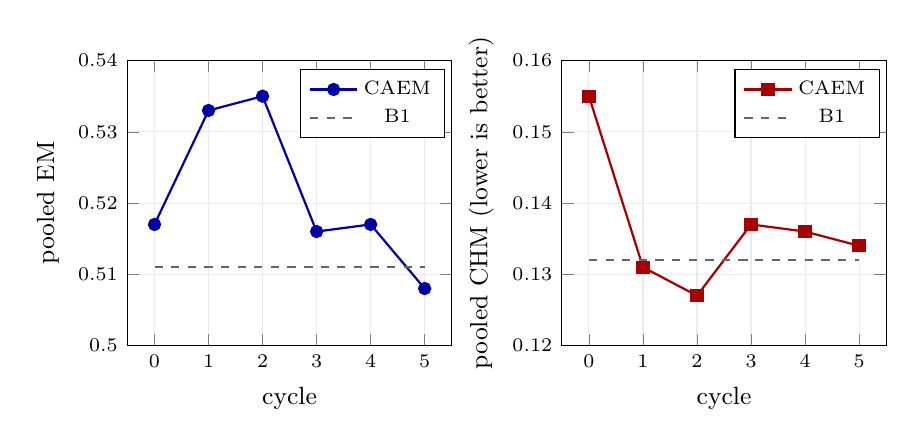
\begin{tikzpicture}
\begin{axis}[name=em, width=0.47\textwidth, height=5.2cm, xlabel={cycle}, ylabel={pooled EM}, xtick={0,...,5},
  ymin=0.50, ymax=0.54, font=\small, tick label style={font=\scriptsize}, grid=major, grid style={black!8},
  legend style={font=\scriptsize, at={(0.98,0.97)}, anchor=north east}]
  \addplot[blue!65!black, mark=*, thick] coordinates {(0,0.517) (1,0.533) (2,0.535) (3,0.516) (4,0.517) (5,0.508)};
  \addlegendentry{CAEM}
  \addplot[black!60, dashed, thick, domain=0:5] {0.511};
  \addlegendentry{B1}
\end{axis}
\begin{axis}[at={(em.east)}, anchor=west, xshift=1.4cm, width=0.47\textwidth, height=5.2cm, xlabel={cycle},
  ylabel={pooled CHM (lower is better)}, xtick={0,...,5}, ymin=0.12, ymax=0.16, font=\small,
  tick label style={font=\scriptsize}, grid=major, grid style={black!8},
  legend style={font=\scriptsize, at={(0.98,0.97)}, anchor=north east}]
  \addplot[red!65!black, mark=square*, thick] coordinates {(0,0.155) (1,0.131) (2,0.127) (3,0.137) (4,0.136) (5,0.134)};
  \addlegendentry{CAEM}
  \addplot[black!60, dashed, thick, domain=0:5] {0.132};
  \addlegendentry{B1}
\end{axis}
\end{tikzpicture}
\caption[EM and CHM by cycle against B1.]{Pooled EM (left) and CHM (right) by cycle on the evaluation fold, against B1. EM is level with B1 at C0, peaks at C2 and returns to B1's level by C5; CHM is above B1 at C0, where the system refuses too often, about level with it from C1, and ends just above it.}
\label{fig:trajectory}
\end{figure}
